% Intended LaTeX compiler: xelatex
\documentclass[aspectratio=149,11pt,italian]{beamer}
\usepackage{graphicx}
\usepackage{longtable}
\usepackage{wrapfig}
\usepackage{rotating}
\usepackage[normalem]{ulem}
\usepackage{amsmath}
\usepackage{amssymb}
\usepackage{capt-of}
\usepackage{icomma}
\usepackage{hyperref}
\institute{Università di Siena}
\usepackage{localheader}
\usepackage{tikz}
\usepackage{booktabs,tabularx,tabularray}
\usepackage{setspace}
\usepackage{quoting}
\usepackage[italian]{babel}
\usepackage{fancybox}
\newcolumntype{R}{>{\raggedleft\arraybackslash}X}
\newcommand\EMTR{\text{EMTR}}
\newcommand{\sumt}[2]{\sum_{t=1}^{+\infty}\dfrac{#1}{\left(#2\right)^t}}
\usetheme{default}
\author{Massimo D'Antoni}
\date{2023-2024}
\title{La tassazione\newline dei redditi societari}
\subtitle{Scienza delle Finanze}
\hypersetup{
 pdfauthor={Massimo D'Antoni},
 pdftitle={La tassazione dei redditi societari},
 pdflang={Italian}}
\begin{document}

\maketitle

\section{La tassazione delle società}


%%%%%%%%%%%%%%%%%%%%%%%%%%%%%%%%%%%%%%%%%%%%%%%%%%%%%%%%%
\begin{frame}{Le forme giuridiche per l'attività di impresa}
\begin{itemize}
\item Nella \alert{società di persone} (\emph{partnership}) i soci rispondono delle
obbligazioni sociali illimitatamente con il proprio patrimonio personale.
Il trasferimento delle quote è difficile e meno frequente.
\item Nella \alert{società per azioni} (\emph{corporation}) la responsabilità dei soci è
limitata al capitale sociale e le quote sono facilmente scambiabili,
specialmente nel caso di società quotate.
\end{itemize}
Queste differenze si riflettono sul trattamento lOfiscale:
\begin{itemize}
\item Le società di persone sono «trasparenti» (\emph{pass-through entity}): il loro
reddito è imputato ai soci (in Italia è assoggettato a IRPEF) in proporzione
alla loro quota e incluso nelle rispettive basi imponibili anche quando non
distribuito.
\item Le società per azioni sono assoggettate all'\alert{imposta societaria} e i soci
pagano l'imposta sugli utili solo quando questi vengono distribuiti. In
Italia l'imposta societaria è denominata \alert{IRES}, Imposta sul reddito
societario.
\end{itemize}
\end{frame}

%%%%%%%%%%%%%%%%%%%%%%%%%%%%%%%%%%%%%%%%%%%%%%%%%%%%%%%%%
\begin{frame}{La rilevanza dell'IRES nei paesi OCSE}
\begin{figure}
\centering
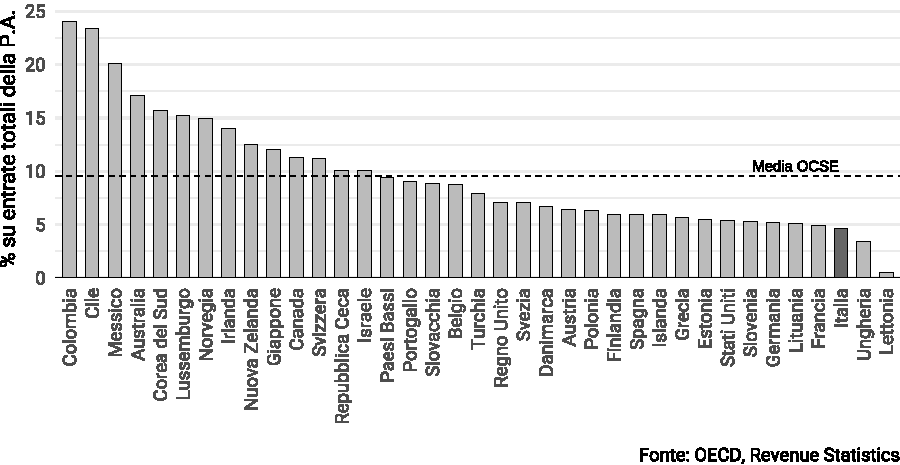
\includegraphics[width=\textwidth]{./figure/imposte-societarie-gettito.pdf}
\caption{Il gettito delle imposte sui redditi societari in \% delle entrate (anno 2019)}
\end{figure}
\end{frame}

%%%%%%%%%%%%%%%%%%%%%%%%%%%%%%%%%%%%%%%%%%%%%%%%%%%%%%%%%
\begin{frame}{Perché una tassazione autonoma delle società di capitali?}
\begin{itemize}
\item \alert{Equità.} Corrispettivo di beni pubblici fruiti dall'impresa nel Paese
(principio del beneficio). Un argomento particolarmente valido quando gli
investitori non sono residenti.
\begin{itemize}
\item Ma allora perché non si applica a tutte le imprese?
\end{itemize}
Corrispettivo per il beneficio specifico della responsabilità limitata
(personalità giuridica) che conferisce una capacità aggiuntiva.
\begin{itemize}
\item Argomento coerente con il fatto che in Italia ad IRES sono assoggettate
anche le S.r.l. e le S.A.p.A. Ma perché tale beneficio sarebbe
proporzionale al reddito?
\end{itemize}
\item \alert{Utilità}. La presenza di un'imposta autonoma sulle società fornisce uno
strumento di politica fiscale in grado di perseguire obiettivi
(es. incentivo all'investimento, allo svolgimento di certe attività\ldots{})
\begin{itemize}
\item In linea di principio si potrebbero utilizzare altri strumenti
incentivanti, anche nel caso di tassazione per trasparenza.
\end{itemize}
\end{itemize}
\end{frame}

%%%%%%%%%%%%%%%%%%%%%%%%%%%%%%%%%%%%%%%%%%%%%%%%%%%%%%%%%
\begin{frame}{Perché una tassazione autonoma delle società di capitali? /2}
\begin{itemize}
\item \alert{Necessità.} La tassazione per trasparenza non è praticabile quando il
numero di soci è elevato e le quote sono scambiate con frequenza.
\item Un'alternativa potrebbe essere quella di limitarsi a tassare l'utile al
momento della sua distribuzione ai soci.
\item Per evitare che tale soluzione si risolva in un incentivo a differire la
tassazione rinviando la distribuzione degli utili, occorre prevedere la
tassazione delle plusvalenze maturate.
\end{itemize}
\begin{block}{}
\small
Una SpA con patrimonio di 10 milioni di euro (un milione di azioni
del valore unitario di 10 €) realizza un utile di un milione di euro.

Se non distribuisce gli utili, il patrimonio aumenta a 11 milioni e il
valore di ciascuna azione aumenta a 11 € (plusvalenza di 1 €). \emph{Se la
plusvalenza è tassata alla maturazione} l'imposta è la stessa che si avrebbe
in caso di distribuzione dei dividendi.

Nota bene: Se successivamente l'impresa distribuirà quell'euro di
cutile, vi sarà un dividendo di 1 € «compensato» da una minusvalenza di 1 €.
\end{block}

\end{frame}

%%%%%%%%%%%%%%%%%%%%%%%%%%%%%%%%%%%%%%%%%%%%%%%%%%%%%%%%%
\begin{frame}{Perché una tassazione autonoma delle società di capitali? /3}
\begin{itemize}
\item La tassazione delle plusvalenze è quasi sempre alla realizzazione. Ciò
  consente il differimento dell'imposta.
\item Dunque, si rende necessaria un'imposta che faccia da \emph{backstop},
  misura di sicurezza per evitare che i soci sfuggano alla
  tassazione. L'imposta sul reddito societario opera dunque come una sorta di
  ritenuta d'acconto.
\end{itemize}
\bigskip

\begin{itemize}
\item Troviamo una conferma indiretta che la differenza tra le diverse forme
  di impresa sia la difficoltà di applicare la trasparenza in presenza di
  azionariato diffuso nel fatto che:
\begin{itemize}
\item In Italia possono optare per la tassazione per trasparenza: le Srl con
  numero di soci non superiore a 10, le società cooperative con numero di
  soci non superiore a 20 (se reddito entro certi limiti), le SpA partecipate
  ad altre società, purché ciascuna di esse abbia partecipazione agli utili e
  diritti di voto tra 10 e 50\%.
\item Negli Stati Uniti possono optare per lo status di S-corporation ed
  essere tassate per trasparenza le società con meno di 100 soci, se questi
  sono residenti.
\end{itemize}
\end{itemize}
\end{frame}

%%%%%%%%%%%%%%%%%%%%%%%%%%%%%%%%%%%%%%%%%%%%%%%%%%%%%%%%%
\begin{frame}{Tipologie di impresa e tassazione: riassumendo}

Tre categorie di imprese residenti:
\begin{itemize}
\item imprese individuali e familiari $\to$ Irpef
\begin{itemize}
\item se impresa familiare, imputabile ai familiari (coniuge, parenti, affini)
fino al 49\% del reddito
\end{itemize}
\item società di persone $\to$ Irpef (applicata ai soci «per trasparenza»)
\begin{itemize}
\item redditi «imputati a ciascun socio, indipendentemente dalla percezione,
proporzionalmente alla sua quota di partecipazione agli utili»
\end{itemize}
\item società di capitali ed enti pubblici e privati $\to$ Ires
\end{itemize}

\begin{block}{}
\begin{center}\small
\begin{tabular}{{lrrr}}
Tipo & numerosità & volume d'affari & reddito d'impresa\\[0pt]
\hline
Imprese individuali & 58\% & 7,9\% & 20,3\%\\[0pt]
Società di persone & 23\% & 9,6\% & 15,2\%\\[0pt]
Società di capitali & 19\% & 82,5\% & 64,5\%\\[0pt]
\end{tabular}
\end{center}
\end{block}
\begin{itemize}
\item Tutti i redditi conseguiti da enti commerciali soggetti IRES e IRPEF
  (imprese individuali e società di persone), da qualsiasi fonte (es. da
  fabbricati, di capitale), sono considerati reddito di impresa.
\end{itemize}
\end{frame}

%%%%%%%%%%%%%%%%%%%%%%%%%%%%%%%%%%%%%%%%%%%%%%%%%%%%%%%%%
\begin{frame}{L'IRES (Imposta sui redditi societari)}
\begin{itemize}
\item \alert{Presupposto} è il possesso di redditi in denaro o in natura da parte dei
seguenti \alert{soggetti passivi}:
\begin{itemize}
\item Gli enti commerciali residenti, siano essi società di capitali (SpA, Srl,
Sapa, ecc.), società cooperative e di mutua assicurazione, enti pubblici e
privati diversi dalle società che esercitano in via esclusiva o principale
un'attività commerciale nel territorio dello Stato. Per tali soggetti il
reddito è considerato in ogni caso reddito di impresa.
\item Gli enti non commerciali residenti, pubblici e privati diversi dalle
società. Il reddito è la somma di redditi fondiari, di capitale, di
impresa e diversi.
\item Società ed enti di ogni tipo, con o senza personalità giuridica, \emph{non
residenti}, per i redditi prodotti in Italia (con criteri vari a seconda
del soggetto e della presenza di una «stabile organizzazione»).
\end{itemize}
\item \alert{Base imponibile} è  il \alert{reddito d’impresa} = Utile/perdita risultante dal
conto economico (codice civile) corretto per tener conto delle variazioni
in aumento e in diminuzione previste dalla normativa fiscale.
\item \alert{Aliquota:} 24\%.
\end{itemize}
\end{frame}

%%%%%%%%%%%%%%%%%%%%%%%%%%%%%%%%%%%%%%%%%%%%%%%%%%%%%%%%%
\begin{frame}{La determinazione contabile del reddito di impresa}
\begin{itemize}
\item Il bilancio a fini fiscali è diverso dal bilancio civilistico.
Perseguono finalità diverse: il bilancio fiscale deve assicurare il
coordinamento tra le imposte, limitare erosioni della base imponibile e
distorsioni nelle scelte di impresa.
\item L'approccio seguito in Europa continentale è quello del «binario unico» o
\emph{uniform reporting}: si parte dal bilancio civilistico e lo si «corregge»
\begin{itemize}
\item Nei paesi anglosassoni l'approccio è quello del «doppio binario» o
\emph{separate reporting}
\end{itemize}
\item Rispetto al bilancio civilistico si apportano alcune variazioni in aumento o
in diminuzione. Le principali differenza dal bilancio civilistico
riguardano:
\begin{itemize}
\item gli interessi passivi
\item i dividendi, le plusvalenze e minusvalenze percepite dalla società
\item gli ammortamenti
\end{itemize}
\item Finalità:
\begin{enumerate}
\item evitare la doppia tassazione del reddito
\item limitare il rischio di elusione
\item evitare effetti distorsivi sulle scelte dell'impresa
\end{enumerate}
\end{itemize}
\end{frame}


%%%%%%%%%%%%%%%%%%%%%%%%%%%%%%%%%%%%%%%%%%%%%%%%%%%%%%%%%
\begin{frame}{La determinazione contabile del reddito di impresa /2}
\begin{center}
\centering
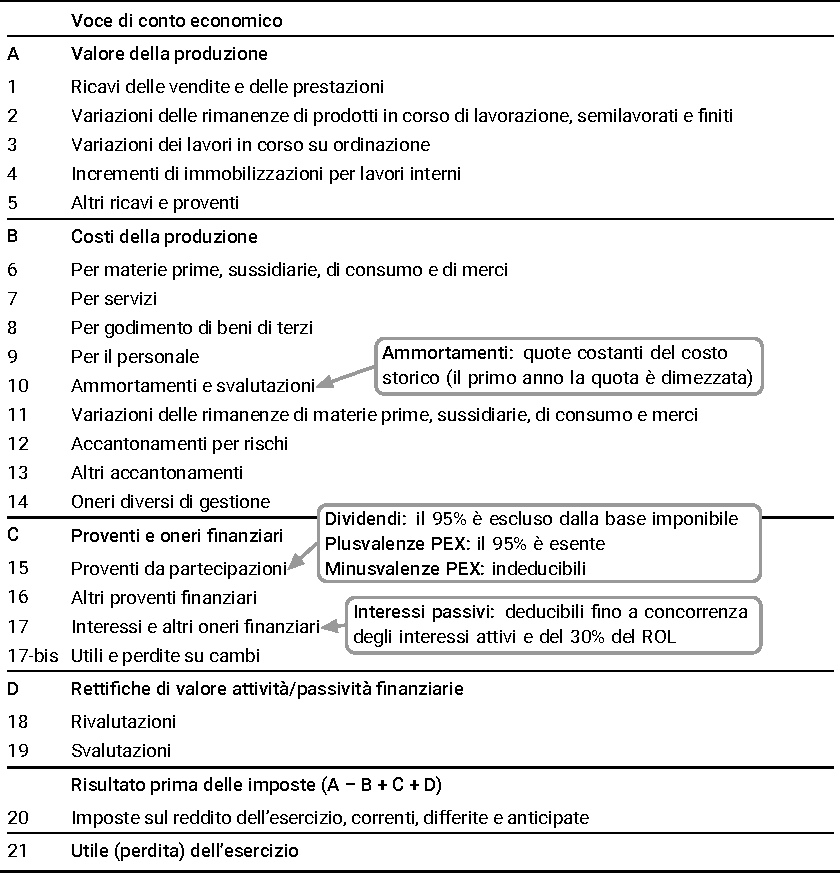
\includegraphics[height=7.5cm]{./figure/tabella-conto-economico.pdf}
\end{center}
\end{frame}

%%%%%%%%%%%%%%%%%%%%%%%%%%%%%%%%%%%%%%%%%%%%%%%%%%%%%%%%%
\begin{frame}{1. Evitare la doppia tassazione del reddito}
\begin{center}
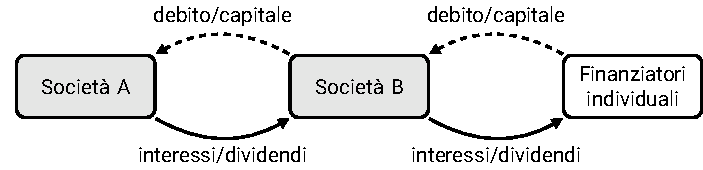
\includegraphics[height=2cm]{./figure/flussi-finanziari.pdf}
\end{center}

\begin{itemize}
\item Se il finanziamento è tramite capitale di rischio, in assenza di correttivi
l'utile viene tassato 3 volte, in capo ad A, a B e agli investitori.
\item Il problema non si presenta nel caso di finanziamento a debito, visto che le
due società avrebbero registrato gli interessi come un costo.
\item La soluzione: i dividendi che una società percepisce dalla partecipazione in
un'altra società sono esenti da imposta per il 95\% (il 5\% residuo si suppone
compensato dai costi di gestione della partecipazione)
\begin{itemize}
\item Eccezione: quando la società A risiede in un paese «a fiscalità
privilegiata»
\end{itemize}
\end{itemize}
\end{frame}


%%%%%%%%%%%%%%%%%%%%%%%%%%%%%%%%%%%%%%%%%%%%%%%%%%%%%%%%%
\begin{frame}{1. Evitare la doppia tassazione del reddito /2}
\begin{itemize}
\item Analoga disposizione per le plusvalenze (\alert{participation exemption, PEX}), al
fine di evitare che vi sia disparità di trattamento nel caso di utili
portati a riserva nella società A e vendita della partecipazione da parte
della società B.
\item La PEX (introdotta in Italia nel 2004) si applica a certe condizioni:
\begin{itemize}
\item possesso della partecipazione ininterrotto per almeno 12 mesi
\item partecipazione classificata come immobilizzazione finanziaria
\item la partecipata svolge effettivamente attività commerciale e non è
residente in paradiso fiscale
\end{itemize}
In assenza di (una di) queste condizioni, le plusvalenze vengono
integralmente tassate e le minusvalenze riconosciute.
\item \emph{dividend washing}: sfrutta la differenza di trattamento tra plusvalenze e
dividendi
\begin{itemize}
\item minusvalenze indeducibili se eccedono i dividendi esenti e realizzate
entro 36 mesi dalla distribuzione dei dividendi
\end{itemize}
\end{itemize}
\end{frame}

%%%%%%%%%%%%%%%%%%%%%%%%%%%%%%%%%%%%%%%%%%%%%%%%%%%%%%%%%
\begin{frame}{Esempio di \emph{dividend washing}}
\begin{itemize}
\item Impresa A produce utile di 1.000 su una partecipazione di 10.000
\item Caso 1: l'utile, distribuito come dividendo alla società B, viene tassato in
capo a B solo per il 5\%
\item Caso 2: la società B cede la sua quota a C prima dello stacco del dividendo
\begin{itemize}
\item prezzo di vendita 11.000
\item la società C riceve il dividendo
\item la società B riacquista la quota da C al prezzo di 10.000
\end{itemize}
\item Dal punto di vista fiscale:
\begin{itemize}
\item per B plusvalenza PEX, esente al 95\%
\item per C dividendi esenti al 95\%
\item per C la minusvalenza non è PEX, dunque dà diritto a una deduzione dal
reddito imponibile
\end{itemize}
\item Soluzione: indeducibilità delle minusvalenze che eccedono i dividendi se
realizzate entro 36 mesi dalla distribuzione dei dividendi
\end{itemize}
\end{frame}

%%%%%%%%%%%%%%%%%%%%%%%%%%%%%%%%%%%%%%%%%%%%%%%%%%%%%%%%%
\begin{frame}{2. Limitare l'elusione - Gli ammortamenti}
\begin{itemize}
\item Possibile ridurre il carico fiscale posticipando il pagamento dell'imposta.
In assenza di vincoli l'impresa potrebbe manipolare la distribuzione
temporale della deduzione per ammortamenti di beni strumentali.
\item La normativa impone regole di deduzione.
\begin{itemize}
\item \alert{Ammortamento a quota costanti} (\emph{straight line}).
\item \alert{Ammortamento a quote decrescenti} (\emph{declining balance}, progressione geometrica)
\end{itemize}
\item La somma delle quote è pari al costo di acquisto (costo storico), ma il
fatto che le deduzioni siano riconosciuti in periodi successivi determina una
divergenza tra costo storico e valore attualizzato delle quote di
ammortamento.
\item In Italia:
\begin{itemize}
\item ammortamento a quote costanti, con quote definite dal MEF per tipologie di
beni. Nell'anno di acquisto la quota è ridotta al 50\%;
\item ammortamento integrale per cassa per beni fino a 516,46€.
\end{itemize}
\end{itemize}
\end{frame}

%%%%%%%%%%%%%%%%%%%%%%%%%%%%%%%%%%%%%%%%%%%%%%%%%%%%%%%%%
\begin{frame}{2. Limitare l'elusione - Gli ammortamenti /2}
\begin{itemize}
\item Ammortamento di un bene acquistato a 1.000 in 5 periodi: confronto tra il
sistema a quote decrescenti e il sistema a quote costanti
\end{itemize}

\medskip
\footnotesize
\begin{tabularx}{\textwidth}{lRR@{\;}RR}
& \multicolumn{2}{c}{Quote decrescenti (40\%)}
& \multicolumn{2}{c}{Quote costanti (20\%)} \\
 & Valore residuo & Ammortamento & Valore residuo & Ammortamento \\
 \midrule
 Periodo 1 & 1.000 & 500 & 1.000 & 200 \\
 Periodo 2 & 500 & 250 & 800 & 200 \\
 Periodo 3 & 250 & 125 & 600 & 200 \\
 Periodo 4 & 125 & 62,25 & 400 & 200 \\
 Periodo 5 & 62,25 & 62,25 & 200 & 200 \\
 & 0 && 0 &\\
 \bottomrule
\end{tabularx}
\begin{itemize}
\item Il valore attualizzato delle quote (interesse 10\%):
\begin{gather*}
\text{Quote decrescenti:}\quad
 \frac{500}{1,1}+\frac{250}{1,1^2}+\frac{125}{1,1^3}+
 \frac{62,25}{1,1^4}+\frac{62,25}{1,1^5}=836,57 \\
\text{Quote costanti:}\quad
 \frac{200}{1,1}+\frac{200}{1,1^2}+\frac{200}{1,1^3}+
 \frac{200}{1,1^4}+\frac{200}{1,1^5}=758,16
\end{gather*}
\end{itemize}
\end{frame}

%%%%%%%%%%%%%%%%%%%%%%%%%%%%%%%%%%%%%%%%%%%%%%%%%%%%%%%%%
\begin{frame}{2. Limitare l'elusione - Gli interessi passivi}
\begin{itemize}
\item Nell'ambito di un gruppo multinazionale è possibile utilizzare il debito per
«spostare» i profitti (\emph{profit-shifting}) in paesi a fiscalità privilegiata:
\begin{itemize}
\item societa A in Italia, società B in paradiso fiscale;
\item la società B eroga un prestito alla società A, che a parità di reddito
vede ridursi i propri profitti in misura corrispondente agli interessi
passivi.
\end{itemize}
\item Una soluzione è rappresentata dalle \emph{earning stripping rules}. In Italia:
interessi passivi deducibili nella misura massima degli interessi attivi
aumentati del 30\% del ROL.
\end{itemize}

\begin{example}[]
\small
Un'impresa ottiene un reddito operativo lordo di 30.000 €, percepisce
interessi attivi per 4.000 € e paga interessi passivi per 23.000 €.  Gli
interessi passivi sono deducibili solo in misura pari a: $4.000 + 30\% \cdot30.000
= 13.000$ euro. Gli interessi passivi in eccesso, pari a 10.000 €, potranno
essere dedotti, entro lo stesso limite, negli esercizi successivi non oltre il
quinto.
\end{example}
\end{frame}


%%%%%%%%%%%%%%%%%%%%%%%%%%%%%%%%%%%%%%%%%%%%%%%%%%%%%%%%%
\begin{frame}{3. Non distorcere le scelte - L'ACE}
\begin{itemize}
\item Asimmetria di trattamento tra remunerazione del capitale proprio e
remunerazione degli interessi
\item Rischio di \emph{thin capitalization}
\item Quali rimedi?
\begin{itemize}
\item Limitata deducibilità degli interessi passivi
\item l'Allowance for Capitale Equity (in Italia: Aiuto alla Crescita Economica).
\end{itemize}
\end{itemize}
\begin{block}{L'ACE}
\begin{itemize}
\item Una deduzione calcolata applicando un tasso di rendimento nozionale a una
base determinata dai nuovi apporti di capitale proprio (successivamente al
31/12/2010).
\item Gli incrementi di capitale investito: nuovi apporti di capitale o utili a
riserva.
\end{itemize}
\end{block}
\end{frame}

%%%%%%%%%%%%%%%%%%%%%%%%%%%%%%%%%%%%%%%%%%%%%%%%%%%%%%%%%
\begin{frame}{L'ACE: esempio}
\begin{itemize}
\item Incremento del patrimonio netto (riserve e conferimenti di capitali)
rispetto al 31/12/2010: € 50.000
\item Utile 2019: € 15.000
\item Alla base imponibile ai fini IRES si applica una deduzione pari a:
\begin{equation*}
  50.000 \times 1,3\% = 650
\end{equation*}
\item Risparmio di imposta redditi 2019: $24\% \times 650 = 156$
\item Se nel 2019 accantono a riserve altri € 10.000, nell'anno successivo la
deduzione è:
\begin{equation*}
  (50.000 + 10.000) \times 1,3\% = 780
\end{equation*}
\item Per cui risparmio di imposta sui redditi 2020: $24\% \times 780 = 187.2$
\item L'accantonamento a riserve mi consente di effettuare un investimento,
es. acquisto di macchinario.  La deduzione è analoga a quella che avrei
avuto ricorrendo a finanziamento a debito con interesse del 1,3\%
\item Efficacia ridimensionata dalla riduzione del coefficiente (era 4,75\% nel 2016!)
\end{itemize}
\end{frame}

%%%%%%%%%%%%%%%%%%%%%%%%%%%%%%%%%%%%%%%%%%%%%%%%%%%%%%%%%
\begin{frame}{La determinazione dell'imposta}
\begin{equation*}
  \begin{array}{ll}
    t \times \Big[\; \text{Utile da bilancio}  &\\
      {}+\text{Variazioni in aumento} &\begin{cases}\;\parbox{36mm}{\raggedright\small Interessi passivi indeducibili}\\[3mm]
        \;\parbox{36mm}{\small Ammortamenti superiori\\ai valori fiscali}\\[3mm]
        \;\parbox{36mm}{\small Minusvalenze PEX\\indeducibili}\end{cases}
        \\[12mm]
    {}-\text{Variazioni in diminuzione} &\begin{cases}
        \;\parbox{33mm}{\raggedright\small 95\% dei dividendi e plusvalenze PEX}\end{cases}\\
    {}-\text{Perdite riportabili}  -\text{ACE} \;\Big] &
  \end{array}
\end{equation*}
\centering\bigskip

L'aliquota IRES è del 24\%
\end{frame}

%%%%%%%%%%%%%%%%%%%%%%%%%%%%%%%%%%%%%%%%%%%%%%%%%%%%%%%%%
\begin{frame}{Le perdite riportabili}
IRES: la società potrà compensare l'80\% dell'utile con la perdita del periodo precedente, senza limiti temporali.

\begin{center}\small
\begin{tabular}{lrrrr}
\toprule
Anno                & $i$ & $i+1$ & $i+2$ & $i+3$ \\
\midrule
Utile/Perdita       & $-200$  & 100   & 60    & 100   \\
Perdita compensata  & 0     & $-80$   & $-48$   & $-72$   \\
Perdita riportabile & $-200$  & $-120$  & $-72$   & 0     \\
Imponibile          & 0     & 20    & 12    & 38    \\
\bottomrule
\end{tabular}
\end{center}
\end{frame}

%%%%%%%%%%%%%%%%%%%%%%%%%%%%%%%%%%%%%%%%%%%%%%%%%%%%%%%%%
\begin{frame}{Differenze società di capitali (IRES) / società di persone (IRPEF)}
\begin{itemize}
\item Dividendi e plusvalenze in regime PEX:
\begin{itemize}
\item concorrono alla formazione del reddito per il 58,14\% del loro
ammontare.
\end{itemize}
\item Interessi passivi:
\begin{itemize}
\item ammessi in deduzione solo nella misura del rapporto $R/(R+E)$, dove $R$
sono i ricavi tassabili ed $E$ i redditi esenti. Serve per evitare
possibili forme di arbitraggio fiscale.
\end{itemize}
\item Possibile riportare le perdite in avanti:
\begin{itemize}
\item illimitatamente nel tempo ma non oltre l'80\% del reddito per soggetti Ires
\item per max 5 anni ma possibile compensare per intero per soggetti Irpef (N.B. dal
2019 i soggetti Irpef uniformati ai soggetti Ires)
\end{itemize}
\end{itemize}
\end{frame}

%%%%%%%%%%%%%%%%%%%%%%%%%%%%%%%%%%%%%%%%%%%%%%%%%%%%%%%%%
\begin{frame}{Andamento delle aliquote nel tempo}
\begin{center}
\centering
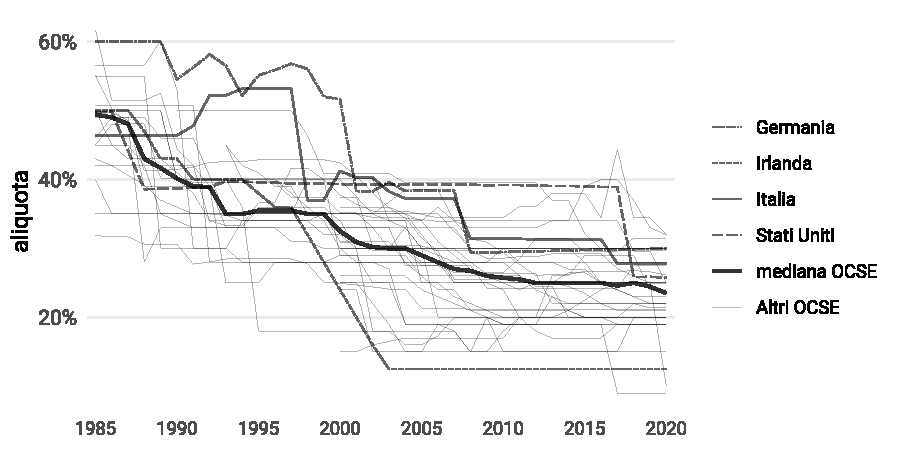
\includegraphics[width=\textwidth]{./figure/aliquote-tassazione-societaria.pdf}
\end{center}
\end{frame}




\section{Le decisioni di investimento dell'impresa}

%%%%%%%%%%%%%%%%%%%%%%%%%%%%%%%%%%%%%%%%%%%%%%%%%%%%%%%%%
\begin{frame}{Effetti dell'imposta societaria sulle decisioni di investimento}
\begin{itemize}
\item L'investimento comporta il sostenimento di un costo e l'ottenimento di un
flusso futuro di profitti
\item Per effettuare l'investimento, necessario approvigionarsi di capitale:
\begin{itemize}
\item tramite un prestito
\item tramite un aumento di capitale
\item con mezzi propri (accantonamento degli utili)
\end{itemize}
\item Dunque la decisione è influenzata da:
\begin{itemize}
\item trattamento fiscale degli utili
\item trattamento fiscale degli ammortamenti
\item trattamento fiscale degli interessi
\item trattamento fiscale degli utili reinvestiti
\end{itemize}
\end{itemize}
\end{frame}

%%%%%%%%%%%%%%%%%%%%%%%%%%%%%%%%%%%%%%%%%%%%%%%%%%%%%%%%%
\begin{frame}{La decisione di investire in assenza di imposte}
\begin{itemize}
\item Consideriamo una politica di investimento che aumenti \alert{permanentemente} di un
ammontare $K$ la dotazione di capitale e in questo modo determini un aumento
permanente del margine operativo (lordo) dell'impresa $\Pi=\Pi(K)$
\item Sia $\delta$ il tasso di usura del capitale investito; il mantenimento del
livello $K$ richiede in ciascun periodo successivo un investimento
aggiuntivo $\delta k$ che mantenga $K$ al livello desiderato
\item L'investimento $K$ risulterà conveniente se $\Pi$ è in grado di garantire
che sia soddisfatta la condizione
\begin{equation*}
 \Pi(K) - \delta K - \rho K\ge 0
\end{equation*}
ovvero: l'incremento nel margine lordo ($\Pi$) deve essere superiore a
quanto necessario per mantenere il livello di capitale ($\delta K$) e per
remunerare i finanziatori ($\rho K$).
\end{itemize}
\end{frame}
%%%%%%%%%%%%%%%%%%%%%%%%%%%%%%%%%%%%%%%%%%%%%%%%%%%%%%%%%
\begin{frame}{L'ottimo livello di investimento: analisi grafica}
\begin{columns}
\begin{column}{.5\columnwidth}
\begin{figure}[htbp]
\centering
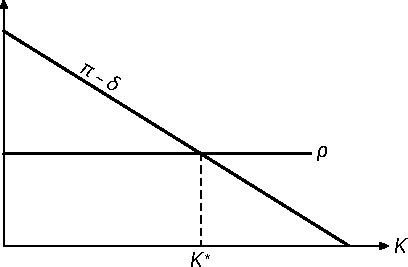
\includegraphics[width=\textwidth]{./figure/scelte-investimento-impresa-1.pdf}
\end{figure}
\end{column}

\begin{column}{.5\columnwidth}
\begin{itemize}
\item Ragionando in termini di variazioni marginali, e quindi indicando con
$\pi=d\Pi/dK$ la variazione marginale del margine operativo lordo, la
condizione di ottimo per l'impresa si può scrivere:
\begin{equation*}
   \pi-\delta - \rho =0
\end{equation*}
\item Nota bene: al crescere di $K$ l'effetto marginale su costi/ricavi misurato
da $\pi=d\Pi/dK$ decresce, e questo spiega l'andamento decrescente della
curva $\pi-\delta$
\end{itemize}
\end{column}
\end{columns}
\end{frame}

%%%%%%%%%%%%%%%%%%%%%%%%%%%%%%%%%%%%%%%%%%%%%%%%%%%%%%%%%
\begin{frame}{È rilevante la struttura finanziaria?}
\begin{itemize}
\item Come varia $\rho$, la remunerazione che va garantita ai finanziatori, al
variare della fonte di finanziamento?
\item In astratto, $\rho$ sarebbe lo stesso per capitale di debito e capitale di
rischio in assenza di incertezza.
\item \alert{Modigliani e Miller}: sotto certe condizioni ideali la struttura
finanziaria non influenza né il valore dell'impresa né il costo del
finanziamento.
\begin{itemize}
\item Intuizione: se aumento l'indebitamento, aumenta il rischio che grava su
ciascuna unità di capitale proprio, ma il valore totale dei due flussi non
varia.
\item La condizione di invarianza di M.-M. vale \alert{in assenza di imposte}. Come
vedremo, l'imposizione può rendere conveniente il ricorso al debito
rispetto al capitale di rischio.
\end{itemize}
\end{itemize}
\end{frame}

%%%%%%%%%%%%%%%%%%%%%%%%%%%%%%%%%%%%%%%%%%%%%%%%%%%%%%%%%
\begin{frame}{Un'imposta sul profitto economico}
\begin{columns}
\begin{column}{.5\columnwidth}
\begin{itemize}
\item Se la base imponibile dell'imposta sul reddito societario coincidesse con il
profitto in senso economico: $\Pi-\delta K - \rho K$, l'imposta non avrebbe
effetto sulle scelte di investimento.
\item Infatti:
$$ \Pi-\delta K - \rho K - t(\Pi-\delta K - \rho K) $$
Riarrangiando e considerando la condizione al margine:
$$ (1-t)(\pi - \delta) = (1-t)\rho $$
\item \alert{Nota bene}: la remunerazione dei finanziatori è dedotta dall'imponibile.
\end{itemize}
\end{column}
\begin{column}{.5\columnwidth}
\begin{center}
\centering
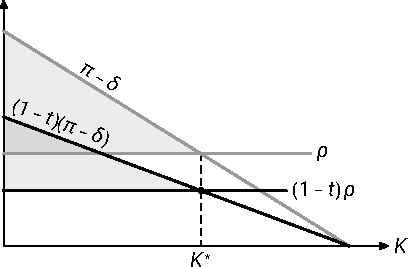
\includegraphics[width=\textwidth]{./figure/scelte-investimento-impresa-2.pdf}
\end{center}
\end{column}
\end{columns}
\end{frame}


%%%%%%%%%%%%%%%%%%%%%%%%%%%%%%%%%%%%%%%%%%%%%%%%%%%%%%%%%
\begin{frame}{Un'imposta sul profitto economico}
\begin{columns}
\begin{column}{.5\columnwidth}
\begin{itemize}
\item Sull'investimento marginale non grava imposta, ma l'imposta colpisce
l'investimento \alert{inframarginale}: il profitto si riduce.
\item Nella realtà la base imponibile differisce dal profitto economico in quanto:
\begin{enumerate}
\item il costo del capitale non è sempre deducibile
\item gli ammortamenti fiscali possono non coincidere con il deprezzamento del
capitale $\delta$
\item la base imponibile è definita in termini nominali (inflazione).
\end{enumerate}
\end{itemize}
\end{column}
\begin{column}{.5\columnwidth}
\begin{center}
\centering
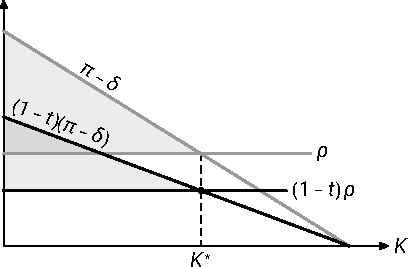
\includegraphics[width=\textwidth]{./figure/scelte-investimento-impresa-2.pdf}
\end{center}
\end{column}
\end{columns}
\end{frame}

%%%%%%%%%%%%%%%%%%%%%%%%%%%%%%%%%%%%%%%%%%%%%%%%%%%%%%%%%
\begin{frame}{Deducibilità parziale dei costi di finanziamento}
\begin{itemize}
\item A seconda della fonte di finanziamento, può essere prevista la deducibilità
totale o parziale dei relativi oneri.
\item Nel caso di tassazione del reddito di impresa, si prevede normalmente:
\begin{itemize}
\item deducibilità degli interessi passivi
\item indeducibilità della remunerazione del capitale di rischio
\end{itemize}
\item Indicando con $\rho$ la remunerazione richiesta dai finanziatori al lordo delle
rispettive imposte, il costo effettivo del finanziamento risulta essere:
\begin{itemize}
\item $(1-t)\rho$ nel caso di finanziamento con debito
\item $\rho$ nel caso di finanziamento con capitale di rischio
\item $(1-c)\rho+c(1-t)\rho=(1-ct)\rho$ nel caso di finanziamento ``misto'', in
parte ($c$) con debito in parte ($1-c$) con capitale di rischio, $0<c<1$
\item in alcuni casi ci sono limiti alla deducibilità degli interessi passivi
\end{itemize}
\end{itemize}

\vspace{-1mm}
\begin{block}{}
\fontsize{8}{9}\selectfont
Ciò che è rilevante è la fonte di finanziamento \emph{al margine}:
\begin{itemize}
\item se ho già utilizzato debito e al margine devo utilizzare capitale
proprio, il finanziamento al margine sarà interamente con capitale proprio
\item se ho raggiunto un rapporto ottimale tra debito e capitale e
voglio aumentare l'investimento mantenendo invariato il rapporto, avrò
finanziamento «misto» al margine.
\end{itemize}
\end{block}
\end{frame}

%%%%%%%%%%%%%%%%%%%%%%%%%%%%%%%%%%%%%%%%%%%%%%%%%%%%%%%%%
\begin{frame}{Deducibilità parziale dei costi di finanziamento: analisi grafica}
\begin{columns}
\begin{column}{.5\columnwidth}
\begin{figure}[htbp]
\centering
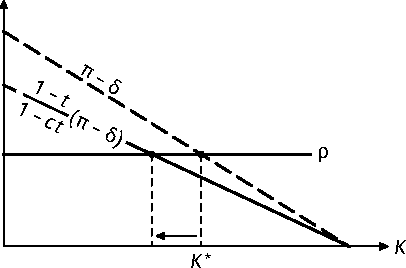
\includegraphics[width=\textwidth]{./figure/scelte-investimento-impresa-4.pdf}
\end{figure}
\end{column}

\begin{column}{.5\columnwidth}
\begin{itemize}
\item Anche a parità di rendimento richiesto dai finanziatori, il trattamento
differenziato dei costi di finanziamento a seconda della fonte incide sulla
decisione di investimento
\item La condizione di scelta al margine risulta così modificata:
\begin{equation*}
   (1-t)(\pi-\delta) = (1-ct)\rho
\end{equation*}
o anche:
\begin{equation*}
   \frac{1-t}{1-ct}(\pi-\delta) = \rho
\end{equation*}
\item Il livello di investimento è inferiore al livello ottimale
\end{itemize}
\end{column}
\end{columns}
\end{frame}

%%%%%%%%%%%%%%%%%%%%%%%%%%%%%%%%%%%%%%%%%%%%%%%%%%%%%%%%%
\begin{frame}{Ammortamento fiscale e ammortamento economico}
\begin{itemize}
\item Le regole fiscali di ammortamento, determinate pre grandi categorie di beni,
normalmente non coincidono con il "vero" deprezzamento del capitale $\delta$
\item Possiamo pensare all'ammortamento fiscale come una riduzione del costo di
acquisto del bene capitale, proporzionale al valore attualizzato delle quote
$A$: $K\to(1-tA)K$.
\item Sia $d_i$ la quota di ammortamento fiscale nel periodo $i$. Abbiamo:
$$ A  = \sum_{i=1}^n\frac{d_i}{\big(1+(1-ct)\rho\big)^i} $$
\item Esempio:
\end{itemize}
\small
\begin{tabularx}{\textwidth}{lcccccc}
  \toprule
  Anno                  & 1    & 2   & 3   & 4   & 5  & Totale \\
  \midrule
   Quota ammortamento & 0,125  & 0,25 & 0,25 & 0,25  & 0,125 & 1\\
   Valori attualizzati & 0,116 &	0,216 &	0,201 &	0,187 &	0,087  & \emph{A} = 0,806  \\
  \toprule
\end{tabularx}
\begin{itemize}
\item L'impresa ottiene una riduzione di imposta pari a $tAK=0,24\times0,806\times K$.
\end{itemize}
\end{frame}

%%%%%%%%%%%%%%%%%%%%%%%%%%%%%%%%%%%%%%%%%%%%%%%%%%%%%%%%%
\begin{frame}{Effetti della deduzione per ammortamenti}
\begin{itemize}
\item Considerando la deduzione per ammortamento abbiamo:
\begin{equation*}
(1-t)\Pi - \delta (1-tA) K - (1-ct)\rho (1-tA) K 
\end{equation*}
da cui la condizione al margine:
\begin{equation*}
(1-t)\pi - (1-tA)\big(\delta + (1-ct)\rho\big) = 0. 
\end{equation*}
\item $A$ dipende dal profilo temporale dell'ammortamento:
\begin{itemize}
\item se fosse $d_i=\delta$ avremmo:
$$ A_\delta = \frac{\delta}{\delta+(1-ct)\rho} $$
\item le analisi empiriche indicano che nella realtà $A>A_\delta$: gli
ammortamenti fiscali sono più generosi dell'ammortamento economico.
\end{itemize}
\item Dato $A\ge A_\delta$, possiamo individuare il valore $0\le a\le 1$ che
risolve: $$ A = (1-a)A_\delta + a $$

Nota bene: $a=1$ quando $A=1$, cioè quando abbiamo una deduzione immediata
del costo del bene strumentale.
\end{itemize}
\end{frame}

%%%%%%%%%%%%%%%%%%%%%%%%%%%%%%%%%%%%%%%%%%%%%%%%%%%%%%%%%
\begin{frame}{Effetti della deduzione per ammortamenti /2}
\begin{equation*}
   (1-t)\pi - (1-at-(1-a)tA_\delta)[\delta + (1-ct)\rho] = 0. 
\end{equation*}
da cui, sostituendo:
\begin{equation*}
  (1-t)(\pi - \delta) - (1-ct)\rho +a t(1-ct)\rho = 0.
\end{equation*}
Raccogliendo infine il termine $(1-ct)$ e dividendo per $(1-ct)(1-at)$, arriviamo a:
\begin{equation*}
  (\pi - \delta) \frac{1-t}{(1-ct)(1-a t)}= \rho.
\end{equation*}
Questa espressione tiene conto della deduzione parziale del costo del capitale $c$ e della divergenza tra ammortamento fiscale ed economico $a$.
\end{frame}


%%%%%%%%%%%%%%%%%%%%%%%%%%%%%%%%%%%%%%%%%%%%%%%%%%%%%%%%%
\begin{frame}{Effective marginal tax rate (EMTR)}
\begin{itemize}
\item Le imposte, riducendo il rendimento effettivo, determinano una divergenze
(cuneo fiscale) tra $\pi-\delta$ e $\rho$. A tale cuneo corrisponde
un'aliquota effettiva (\emph{Effective marginal tax rate (EMTR)}) pari a:
\begin{equation*}
(\pi-\delta)(1-\EMTR)=\rho
\end{equation*}
Dalle formule precedenti l'EMTR risulta
essere:
\begin{equation*}
 \EMTR = 1 - \frac{1-t}{(1-ct)(1-at)}.
\end{equation*}
\item Con questa formula possiamo valutare l'effetto complessivo dell'imposta,
della deducibilità del costo del capitale e degli ammortamenti
\end{itemize}

\begin{center}
\centering
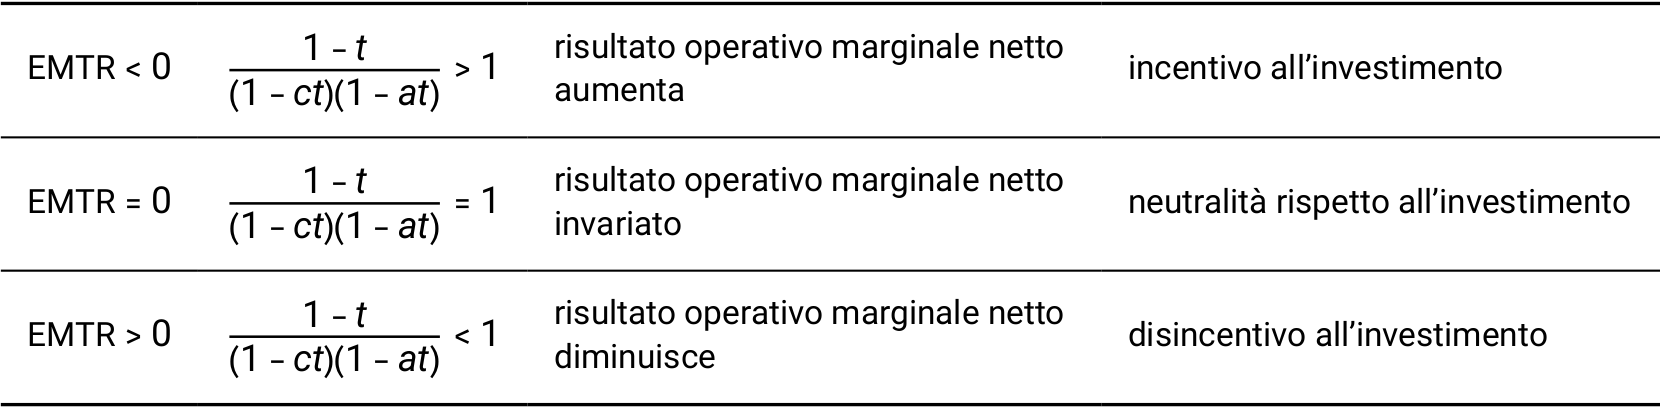
\includegraphics[width=\textwidth]{./figure/EMTR.png}
\end{center}
\end{frame}

%%%%%%%%%%%%%%%%%%%%%%%%%%%%%%%%%%%%%%%%%%%%%%%%%%%%%%%%%
\begin{frame}{Effetti dell'imposta sull'investimento}
\begin{columns}
\begin{column}{.6\columnwidth}
\begin{center}
\centering
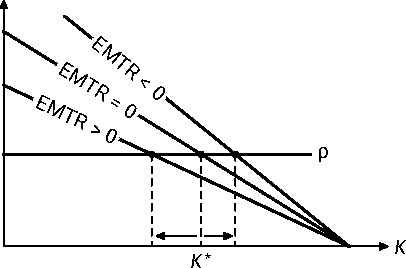
\includegraphics[width=\textwidth]{./figure/scelte-investimento-impresa-5.pdf}
\end{center}
\end{column}

\begin{column}{.4\columnwidth}
L'EMTR può assumere valori positivi o negativi. Quando assume valori positivi determina un sussidio implicito all'investimento    
\end{column}
\end{columns}
\end{frame}

%%%%%%%%%%%%%%%%%%%%%%%%%%%%%%%%%%%%%%%%%%%%%%%%%%%%%%%%%
\begin{frame}{Alcune conclusioni /1}
\begin{itemize}
\item \alert{Le imposte societarie incentivano le imprese a finanziarsi con debito}

Ciò si vede dal fatto che con debito $c>0$, potrebbe essere $c=1$, mentre con capitale di rischio $c=0$.

\item \alert{Quando le imprese si finanziano con debito l'imposta sulle società può incentivare l'investimento}

\begin{equation*}
  \EMTR_{debito}=-\frac{at_s}{1-at_s}
\end{equation*}

L'imposta introduce un sussidio al margine (tanto maggiore quanto più alta è l'imposta!)

\item \alert{Quando le imprese si finanziano con capitale di rischio l'investimento è disincentivato (a meno che la spesa per investimenti non sia immeditamente deducibile)}

Quando $c=0$ per avere neutralità occorre che sia $a=1$
\end{itemize}
\end{frame}


%%%%%%%%%%%%%%%%%%%%%%%%%%%%%%%%%%%%%%%%%%%%%%%%%%%%%%%%%
\begin{frame}{Valori di EMTR stimati}
\begin{center}
\centering
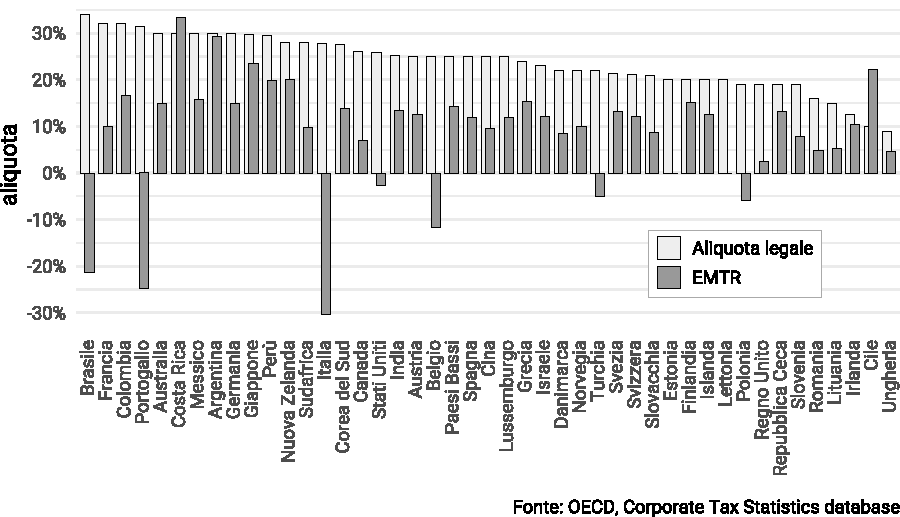
\includegraphics[width=\textwidth]{./figure/EMTR.pdf}
\end{center}
\end{frame}

%%%%%%%%%%%%%%%%%%%%%%%%%%%%%%%%%%%%%%%%%%%%%%%%%%%%%%%%%
\begin{frame}{Come ristabilire la neutralità?}
\begin{itemize}
\item Rimuovere il vantaggio degli interessi passivi (non deducibilità). Questa soluzione è stata ipotizzata nella proposta della \emph{Comprehensive Business Income Tax} (CBIT) americana.
\begin{itemize}
\item Vedi in Italia l'IRAP
\end{itemize}

\item Con $c=0$ (indeducibilità degli interessi) e $a=1$ (immediata deducibilità degli investimenti) abbiamo la \emph{cash-flow tax}.
\begin{itemize}
\item Richiama l'idea di reddito consumo
\item Applicata solo in rari casi (Estonia, Macedonia, Messico) in quanto: ha effetti prociclici, sposta le imposte in avanti portando a una perdita di gettito, pone problemi di coordinamento internazionale.
\end{itemize}

\item Una terza opzione è l'ACE \emph{Allowance for Corporate Equity}, che prevede una deduzione dall'imponibile del costo del capitale anche quando finanziato con capitale di rischio.
\end{itemize}
\end{frame}



%%%%%%%%%%%%%%%%%%%%%%%%%%%%%%%%%%%%%%%%%%%%%%%%%%%%%%%%%
\begin{frame}{L'ACE e la scelta della fonte di finanziamento}
\begin{itemize}
\item Nel caso di finanziamento con capitale di rischio, l'investimento $K$ viene
accompagnato da un aumento di pari ammontare nel patrimonio netto
dell'impresa (ritenzione degli utili oppure aumento del capitale sociale)
--- che si mantiene per tutta la durata dell'investimento
\item In questo caso l'ACE prevede, nei periodi successivi, una deduzione
dall'imponibile pari al profitto ``normale'' derivante dal nuovo capitale
proprio, calcolato come
\begin{equation*}
  [\text{incremento patrimonio netto}] \times [\text{rendimento nozionale}]
\end{equation*}
\item Nel nostro schema, la condizione marginale per la
scelta ottimale diventa:
\begin{equation*}
  \pi - \delta - \rho - t_s (\pi - \delta - \rho_N )=0
\end{equation*}
\item In altre parole, indipendentemente dalla fonte di finanziamento (capitale o
debito) abbiamo piena deducibilità dei costi di finanziamento, e la scelta
della fonte di finanziamento risulta neutrale
\end{itemize}
\end{frame}
\section{L'integrazione tra imposta societaria e imposta del socio}

%%%%%%%%%%%%%%%%%%%%%%%%%%%%%%%%%%%%%%%%%%%%%%%%%%%%%%%%%
\begin{frame}{Integrazione tra imposta del socio e della società di capitali}
\begin{itemize}
\item Nel \alert{sistema della tassazione per trasparenza} l'utile viene imputato pro quota al
socio e tassato come reddito nell'imposta personale (aliquota $t_p$)

\item Con l'imposta sul reddito societario l'utile, dopo essere tassato in capo
alla società (aliquota $t$), viene tassato in capo al socio quando al
momento della distribuzione. L'imposta totale è: $\tau=t + (1-t)t_d$.

Diversi sistemi di integrazione tra le due imposte:
\begin{itemize}
\item \alert{Sistema classico}: tassazione del socio e dell'impresa sono indipendenti.
Ai dividendi si applica la stessa imposta che si applica sugli interessi
$t_d=t_i$ (eventualmente pari all'imposta personale $t_p$).

\item \alert{Sistema classico modificato}: a differenza del sistema classico, sui
dividendi si applica un'imposta inferiore a quella applicata sugli
interessi: $t_d<t_i$.

\item \alert{Sistema di imputazione}: si riconosce al socio un credito per l'imposta
pagata in capo alla società.

\item \alert{Sistema dell'esenzione}: l'utile è tassato solo in capo alla società in
cui viene prodotto.
\end{itemize}
\end{itemize}
\end{frame}

%%%%%%%%%%%%%%%%%%%%%%%%%%%%%%%%%%%%%%%%%%%%%%%%%%%%%%%%%
\begin{frame}{Il sistema classico e il sistema classico modificato}
\begin{itemize}
\item Nel sistema classico l'imposta gravante sui dividendi è $\tau=t+(1-t)t_i$.
\begin{itemize}
\item Se gli interessi sono deducibili dal reddito societario, sugli interessi
grava un'imposta totale $t_i$, inferiore a quella gravante sui dividendi.
\end{itemize}
Questa è la soluzione adottata in Italia, dove $t_i=t_d=0,26$ e $t=0,24$,
per cui sui dividendi grava:
\begin{equation*}
  \tau=0,24 + 0,26(1-0,24)=0,4376
\end{equation*}
mentre per gli interessi è $t_i=0,26$.
\item Nel sistema classico modificato, con $t_d<t_i$, è possibile ottenere il
risultato $t_i=(1-t)t_d$, fissando:
\begin{equation*}
  t_d=\frac{t_i-t}{1-t}
\end{equation*}
È questa la soluzione vigente negli USA, dove $t_i$ è l'imposta personale
sul reddito, mentre \$t\textsubscript{d}<4 segue un diverso sistema di scaglioni. Nel caso
di dividendi: $\tau=0,21 + 0,2(1-0,21)=0,368$, aliquota analoga a quella del
massimo scaglione ($0,37$).
\end{itemize}
\end{frame}

%%%%%%%%%%%%%%%%%%%%%%%%%%%%%%%%%%%%%%%%%%%%%%%%%%%%%%%%%
\begin{frame}{Sistema dell'imputazione}
\begin{itemize}
\item In questo caso si riconosce al socio un credito di imposta per l'imposta
pagata dalla società, per cui: $\tau = t + (t_p-t)=t_p$.
\item È il sistema più coerente con la logica dell'imposta societaria come
"acconto" sull'imposta personale.
\item Il credito può essere comunicato dalla società oppure calcolato a partire
dall'ammontare del dividendo $D$. In questo caso la formula è:
\begin{equation*}
T_d=t_p U -tU
= t_p\left(D+\frac{t}{1-t}D\right)-\frac{t}{1-t}D
= \frac{t_p-t}{1-t}D
\end{equation*}
\item Il sistema è stato progressivamente abbandonato in Europa anche perché
ostacolava la mobilità dei capitali nella UE.
\item Nota bene: alla fine $\tau U = tU + T_d= tU+(t_pU-tU)=t_pU$. Tuttavia
l'equivalenza $\tau=t_p$ non tiene conto del fatto che l'imposta
in capo al socio può essere differita nel tempo.
\end{itemize}
\end{frame}

%%%%%%%%%%%%%%%%%%%%%%%%%%%%%%%%%%%%%%%%%%%%%%%%%%%%%%%%%
\begin{frame}{Evoluzione delle forme di integrazione in Italia}
\begin{itemize}
\item Con l'introduzione dell'Irpeg (1/1/1974) sistema classico
\item immediatamente (luglio 1974) cedolare del 30\%, poi alzata al 50\%
\item dal 1977 al 2003 sistema di imputazione con credito di imposta integrale
\item dal 1994 introdotta possibilità di optare per cedolare del 12,5\%
\item dal 2004 (introduzione Ires al posto dell'Irpeg) il sistema attuale:
\begin{itemize}
\item sistema \emph{cedolare} (ritenuta a titolo definitivo del 26\%)
\item per partecipazioni qualificate fino al 2017 sistema di \emph{esenzione
parziale}: gli utili distribuiti (dividendi) entrano parzialmente nella
base imponibile Irpef
\item possibilità di applicare il \emph{sistema per trasparenza} per:
\begin{itemize}
\item società di capitali partecipate da altre società di capitali (ciascuno dei
quali ha partecipazione non inferiore al 10\%)
\item S.r.l. partecipate da persone fisiche a ristretta base azionaria (max 10
soci, 20 soci se cooperative)  e che rientra nel campo di applicazione
degli studi di settore
\end{itemize}
\end{itemize}
\end{itemize}
\end{frame}
%%%%%%%%%%%%%%%%%%%%%%%%%%%%%%%%%%%%%%%%%%%%%%%%%%%%%%%%%
\begin{frame}{I sistemi di integrazione nei paesi OCSE}
\begin{center}
\centering
\includegraphics[width=\textwidth]{./figure/integrazione-imposta-società-socio.png}
\end{center}
\end{frame}

%%%%%%%%%%%%%%%%%%%%%%%%%%%%%%%%%%%%%%%%%%%%%%%%%%%%%%%%%
\begin{frame}{Come si spiega quel "58,14\%" ?}
La percentuale del 58,14\% per i dividendi percepiti da società di persone e
imprese individuali non è casuale:
\begin{itemize}
\item Utile $U=100$, su cui imposta societaria con aliquota $t=24\%$
\item Se l'utile al netto delle imposte viene distribuito come dividendo, viene
tassato in Irpef solo per il 58,14\%, ovvero
$R=0,5814\cdot(1-t)U=0,5814\cdot76=44,18$
\item Consideriamo un contribuente con reddito superiore a 50.000€: su $R$ si
applica l'aliquota marginale, che in questo caso è quella massima (43\%):
$0,43\cdot44,18\approx19,00$
\item la somma dell'imposta pagata in capo alla società (24) e quella pagata
dal socio (19) dà 43 (43\% dell'utile lordo 100), pari a quello che il socio
avrebbe pagato ad es. in regime di trasparenza.
\begin{itemize}
\item \alert{Nota bene:}
per soci/contribuenti con aliquota marginale dell'Irpef inferiore al 43\%,
l'equivalenza non c'è (si provi a calcolare il carico fiscale con le
aliquote del 41\%, 38\% ecc.)
\end{itemize}
\end{itemize}
\end{frame}

\section{Imposte personali e investimento}


%%%%%%%%%%%%%%%%%%%%%%%%%%%%%%%%%%%%%%%%%%%%%%%%%%%%%%%%%
\begin{frame}{La tassazione sui prestatori di capitale}
\begin{itemize}
\item Finora abbiamo preso per dato $\rho$, la remunerazione \emph{lorda} richiesta dai
finanziatori dell'impresa. Questi sono tuttavia interessati al finanziamento
\emph{netto}, e dunque acquista rilevanza il diverso trattamento fiscale dei vari
canali di finanziamento in capo ai finanziatori stessi
\item Nel caso di \alert{finanziamento con debito} il rendimento netto sarà $(1-t_i)\rho_D=r$,
dove $t_i$ è l'aliquota sugli interessi da obbligazioni o prestiti
\begin{itemize}
\item in Italia attualmente $t_i=26\%$
\end{itemize}
\item Nel caso di \alert{finanziamento con emissione di nuove azioni} il rendimento è
percepito sotto forma di dividendi, e quindi il rendimento netto è $(1-t_d)\rho_{NE}=r$
dove $t_d$ è l'aliquota sui dividendi distribuiti (aggiuntiva rispetto all'imposta
eventualmente pagata dall'impresa sull'utile distribuito)
\end{itemize}
\end{frame}

%%%%%%%%%%%%%%%%%%%%%%%%%%%%%%%%%%%%%%%%%%%%%%%%%%%%%%%%%
\begin{frame}{La tassazione dei prestatori di capitale /2}
\begin{itemize}
\item Nel caso di \alert{finanziamento con reinvestimento degli utili}, i finanziatori
rinunciano ai dividendi oggi per aumentare l'utile domani.
\begin{itemize}
\item Supponiamo che i soci rinuncino oggi a 1€ netto. Ciò comporterà un
investimento aggiuntivo della società pari a $1/(1-t_d)€$, che determinerà
nell'immediato una plusvalenza, tassata con aliquota $t_g$.
\item Quindi a fronte della rinuncia a 1€ di consumo da parte dei soci,
l'investimento dell'impresa sarà $(1-t_g)/(1-t_d)€$.
\item Tale investimento, aumentato del rendimento \$$\rho$\textsubscript{RE}, potrà essere
distribuito (e quindi tassato) nel periodo successivo. Perché l'operazione
risulti conveniente ai soci il rendimento deve essere almeno:
\begin{equation*}
\frac{1-t_g}{1-t_d}\rho_{RE}(1-t_d)=(1-t_g)\rho_{RE}=r
\end{equation*}
per cui:
\begin{equation*}
\rho_{RE}=\frac{r}{1-t_g}
\end{equation*}
\end{itemize}
\item Le imposte sui dividendi non hanno effetto sugli investimenti quando il
finanziamento avviene attraverso utili non distribuiti.
\end{itemize}
\end{frame}

%%%%%%%%%%%%%%%%%%%%%%%%%%%%%%%%%%%%%%%%%%%%%%%%%%%%%%%%%
\begin{frame}{La tassazione sui prestatori di capitale /3}
\begin{center}
\centering
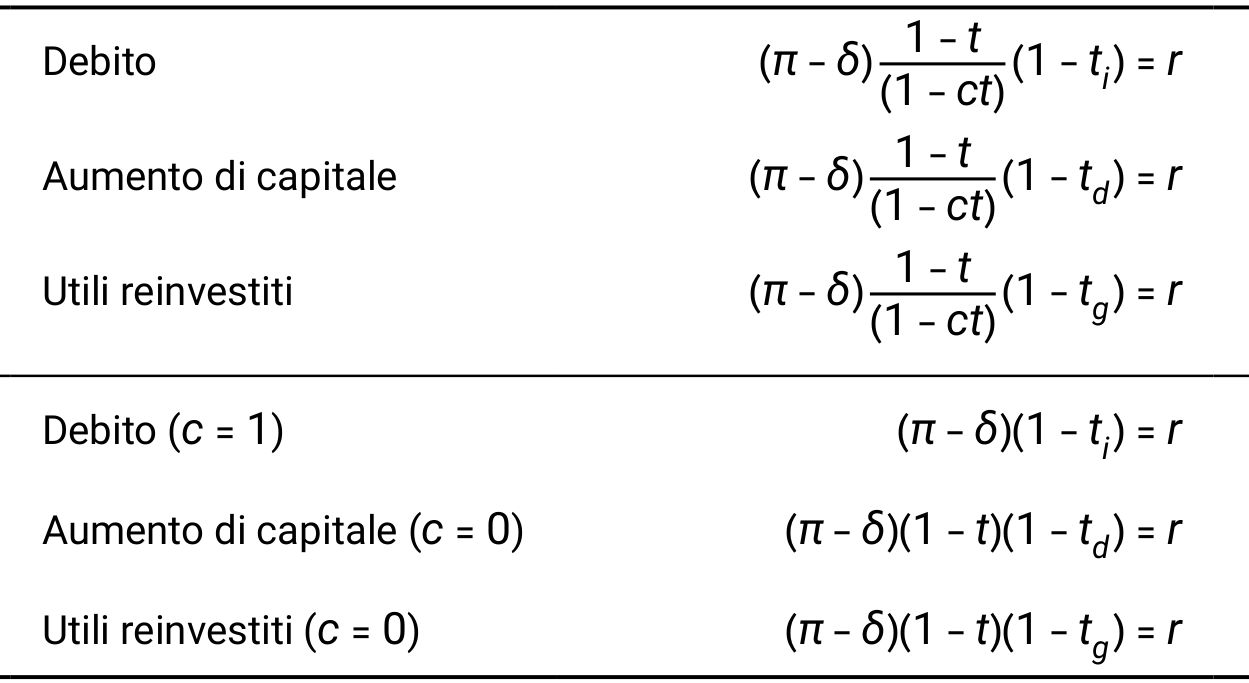
\includegraphics[height=5cm]{./figure/ottimo-investimento-e-fonte-di-finanziamento.png}
\end{center}

\small
\begin{itemize}
\item Con il sistema dell'imputazione o il sistema classico modificato $t_i>t_d$.
D'altra parte, anche se formalmente $t_d=t_g$, la tassazione delle
plusvalenze alla realizzazione determinat un vantaggio fiscale per queste
ultime..
\item Le imposte personali possono riequilibrare l’incentivo al finanziamento con
debito fornito dall’imposta societaria. Quando $(1-t)(1-t_d)=1-t_i$ le due
fonti di finanziamento sono equiparate.
\end{itemize}
\end{frame}
\end{document}